\begin{figure*}[htb]
\begin{minipage}[t]{0.48\linewidth}
\center
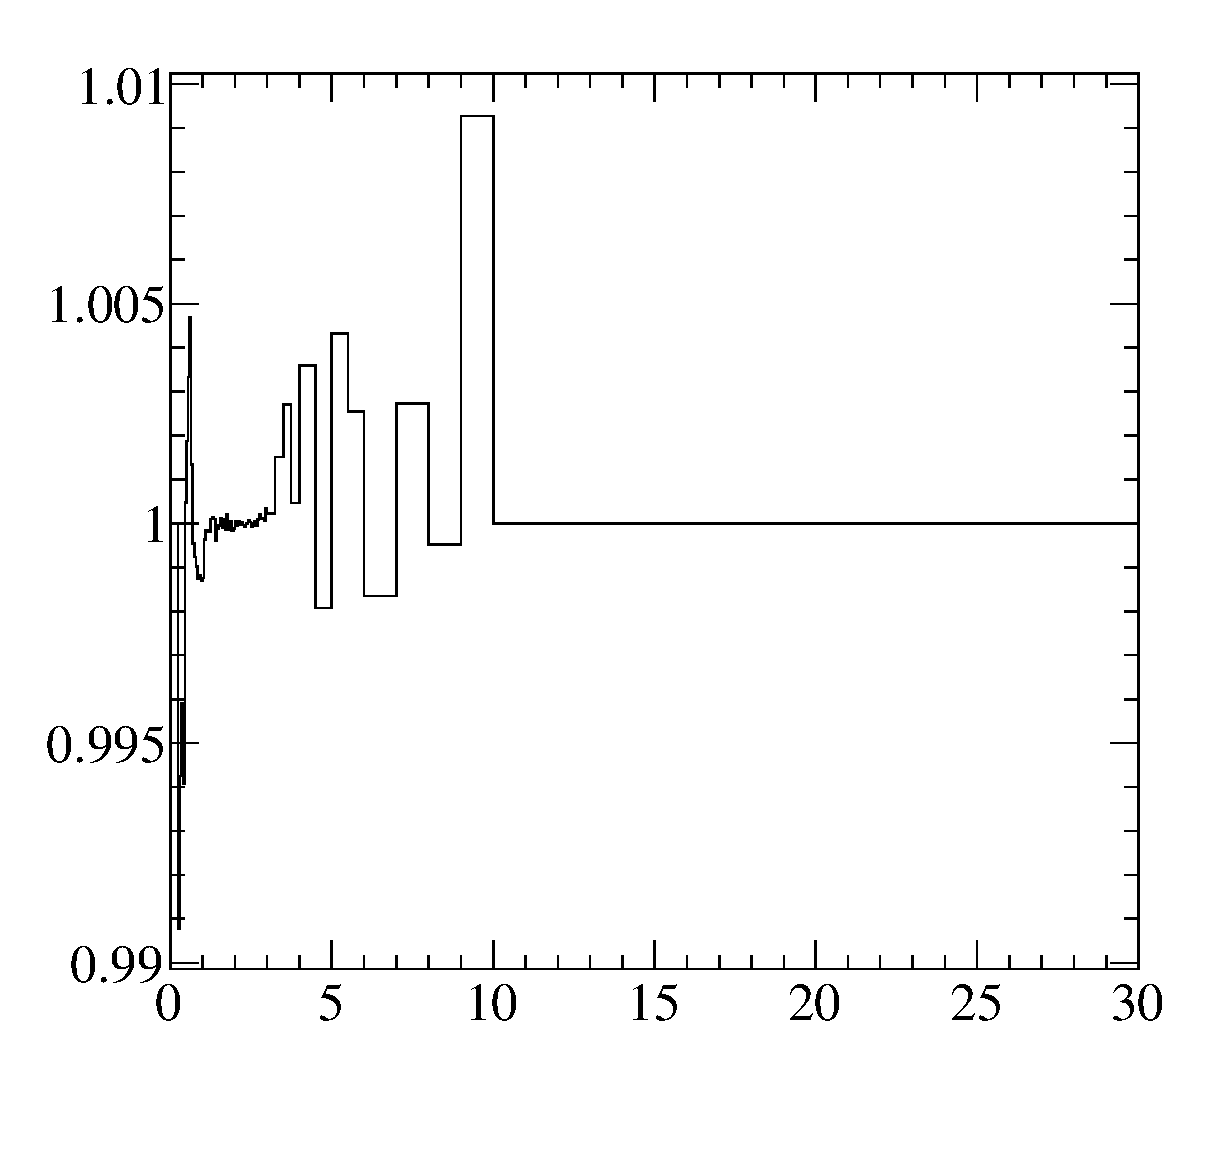
\includegraphics[width=18pc]{./images/binning/oscillation/plot_erec_int_numu_ccqe_fine}
\caption
 {Ratio of SuperK MC $E_{reco}$ spectra, for mode $\nu_\mu$ CCQE made with 84 bin $E_{true}$ and 780 bin $E_{true}$, for an exposure of 3.010$	imes$10$^{20}$ POT. The number of events was calculated using the BANFF-tuned MC templates.Using oscillation parameters:  $\sin^22\theta_{12} = $0.857; $\sin^22\theta_{13} = $0.098; $\sin^22\theta_{23} = $1; $\delta_{CP} = $        0; $\Delta m^2_{21} = $    7.5e-05 $eV^2/c^4$; $|\Delta m^2_{32}| = $    0.0024 $eV^2/c^4$. }
\label{fig:etruebin:numuccqe}
\end{minipage}
\hspace{0.06\linewidth}
\begin{minipage}[t]{0.48\linewidth}
\center
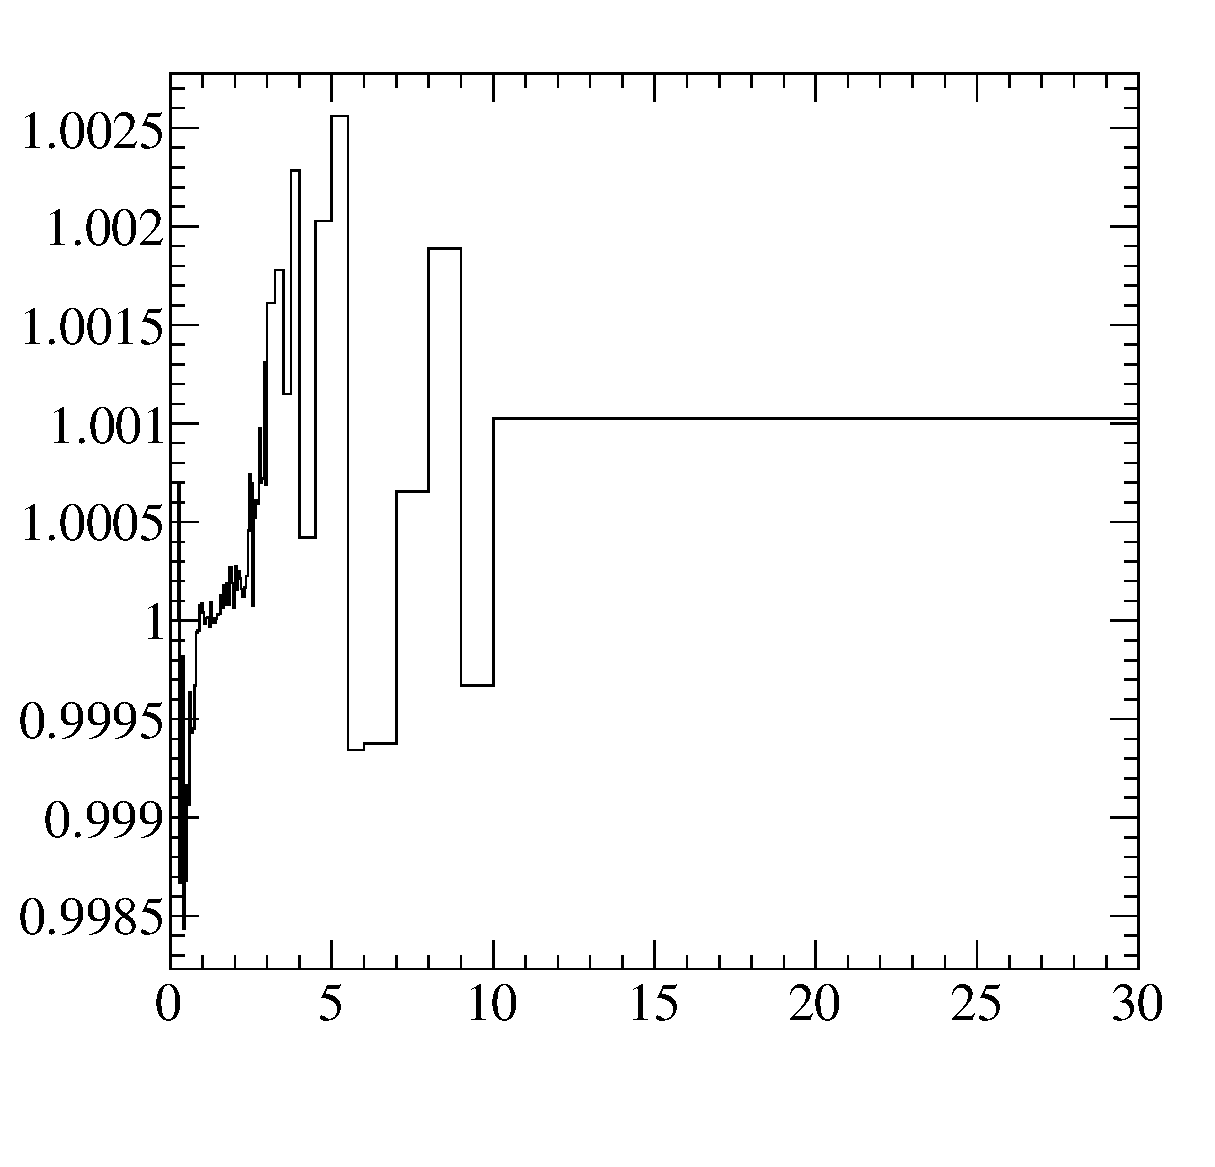
\includegraphics[width=18pc]{./images/binning/oscillation/plot_erec_int_numu_ccpi_fine}
\caption
 {Ratio of SuperK MC $E_{reco}$ spectra, for mode $\nu_\mu$ CC 1$\pi$ made with 84 bin $E_{true}$ and 780 bin $E_{true}$, for an exposure of 3.010$	imes$10$^{20}$ POT. The number of events was calculated using the BANFF-tuned MC templates.Using oscillation parameters:  $\sin^22\theta_{12} = $0.857; $\sin^22\theta_{13} = $0.098; $\sin^22\theta_{23} = $1; $\delta_{CP} = $        0; $\Delta m^2_{21} = $    7.5e-05 $eV^2/c^4$; $|\Delta m^2_{32}| = $    0.0024 $eV^2/c^4$. }
\label{fig:etruebin:numucc1pi}
\end{minipage}
\vfill
\begin{minipage}[t]{0.48\linewidth}
\center
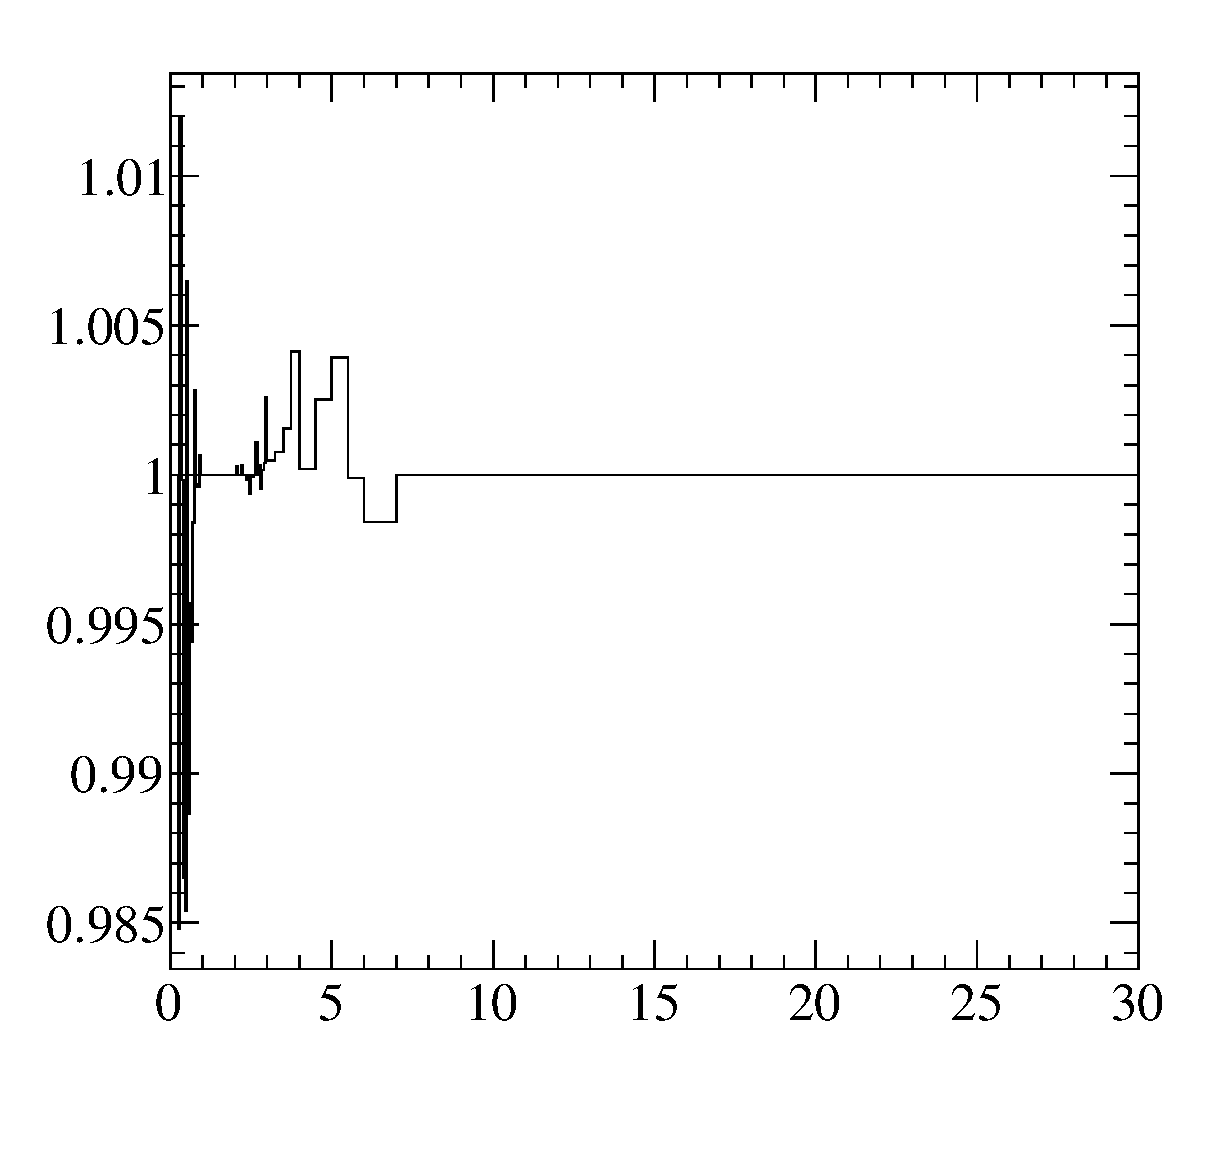
\includegraphics[width=18pc]{./images/binning/oscillation/plot_erec_int_numu_cccoh_fine}
\caption
 {Ratio of SuperK MC $E_{reco}$ spectra, for mode $\nu_\mu$ CC coherent made with 84 bin $E_{true}$ and 780 bin $E_{true}$, for an exposure of 3.010$	imes$10$^{20}$ POT. The number of events was calculated using the BANFF-tuned MC templates.Using oscillation parameters:  $\sin^22\theta_{12} = $0.857; $\sin^22\theta_{13} = $0.098; $\sin^22\theta_{23} = $1; $\delta_{CP} = $        0; $\Delta m^2_{21} = $    7.5e-05 $eV^2/c^4$; $|\Delta m^2_{32}| = $    0.0024 $eV^2/c^4$. }
\label{fig:etruebin:numucccoh}
\end{minipage}
\hspace{0.06\linewidth}
\begin{minipage}[t]{0.48\linewidth}
\center
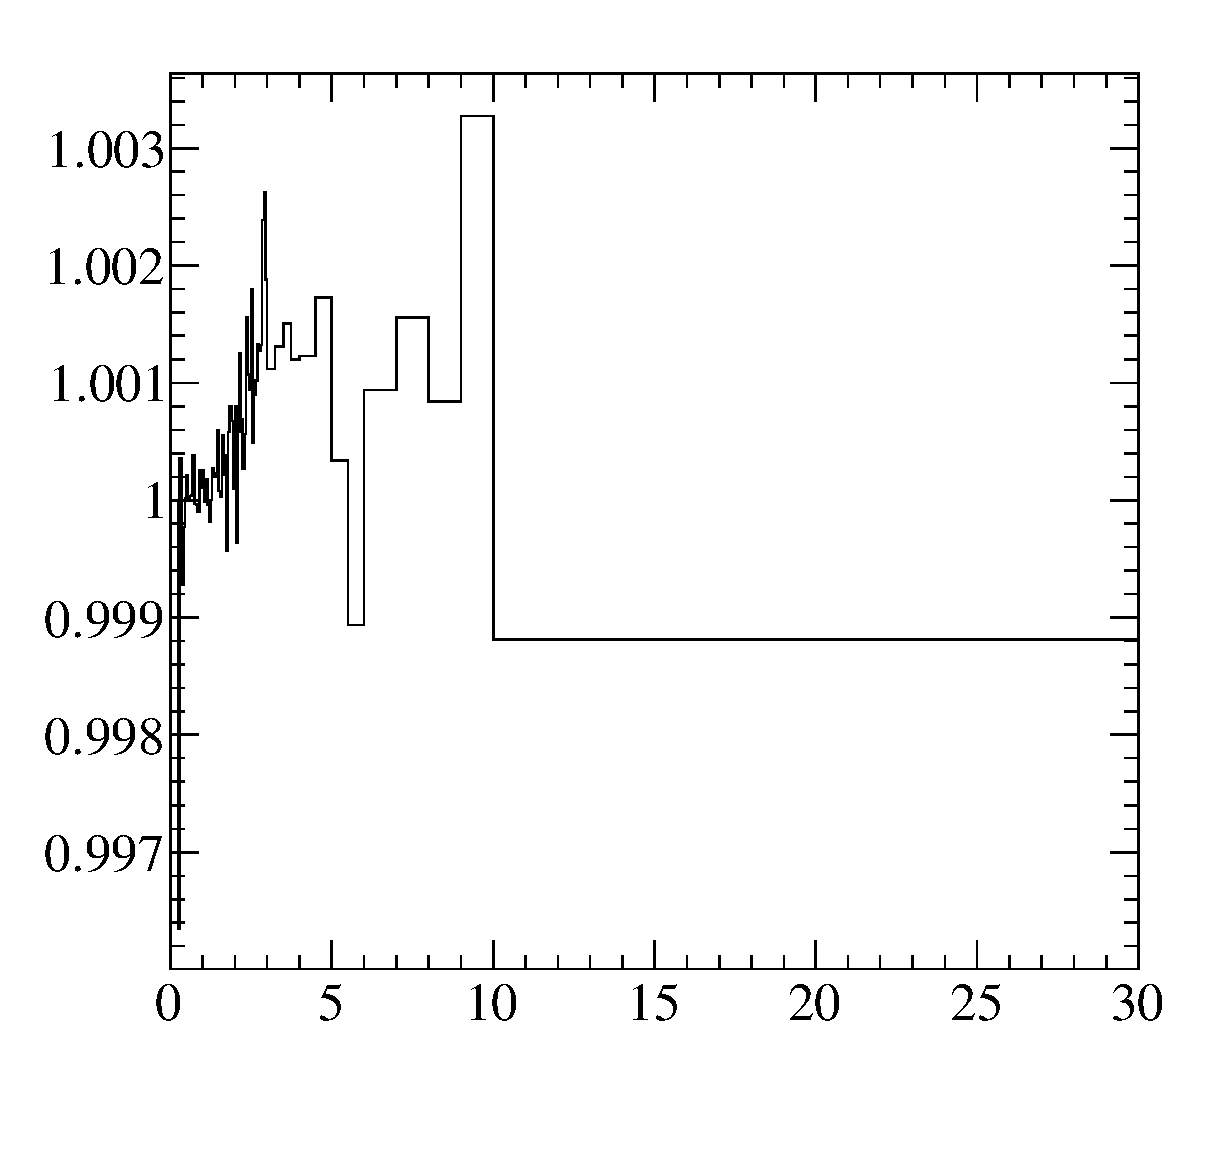
\includegraphics[width=18pc]{./images/binning/oscillation/plot_erec_int_numu_ccoth_fine}
\caption
 {Ratio of SuperK MC $E_{reco}$ spectra, for mode $\nu_\mu$ CC other ($\nu_\mu$ disap) made with 84 bin $E_{true}$ and 780 bin $E_{true}$, for an exposure of 3.010$	imes$10$^{20}$ POT. The number of events was calculated using the BANFF-tuned MC templates.Using oscillation parameters:  $\sin^22\theta_{12} = $0.857; $\sin^22\theta_{13} = $0.098; $\sin^22\theta_{23} = $1; $\delta_{CP} = $        0; $\Delta m^2_{21} = $    7.5e-05 $eV^2/c^4$; $|\Delta m^2_{32}| = $    0.0024 $eV^2/c^4$. }
\label{fig:etruebin:numuccoth}
\end{minipage}
\end{figure*}

%\clearpage
\begin{figure*}[htb]
\begin{minipage}[t]{0.48\linewidth}
\center
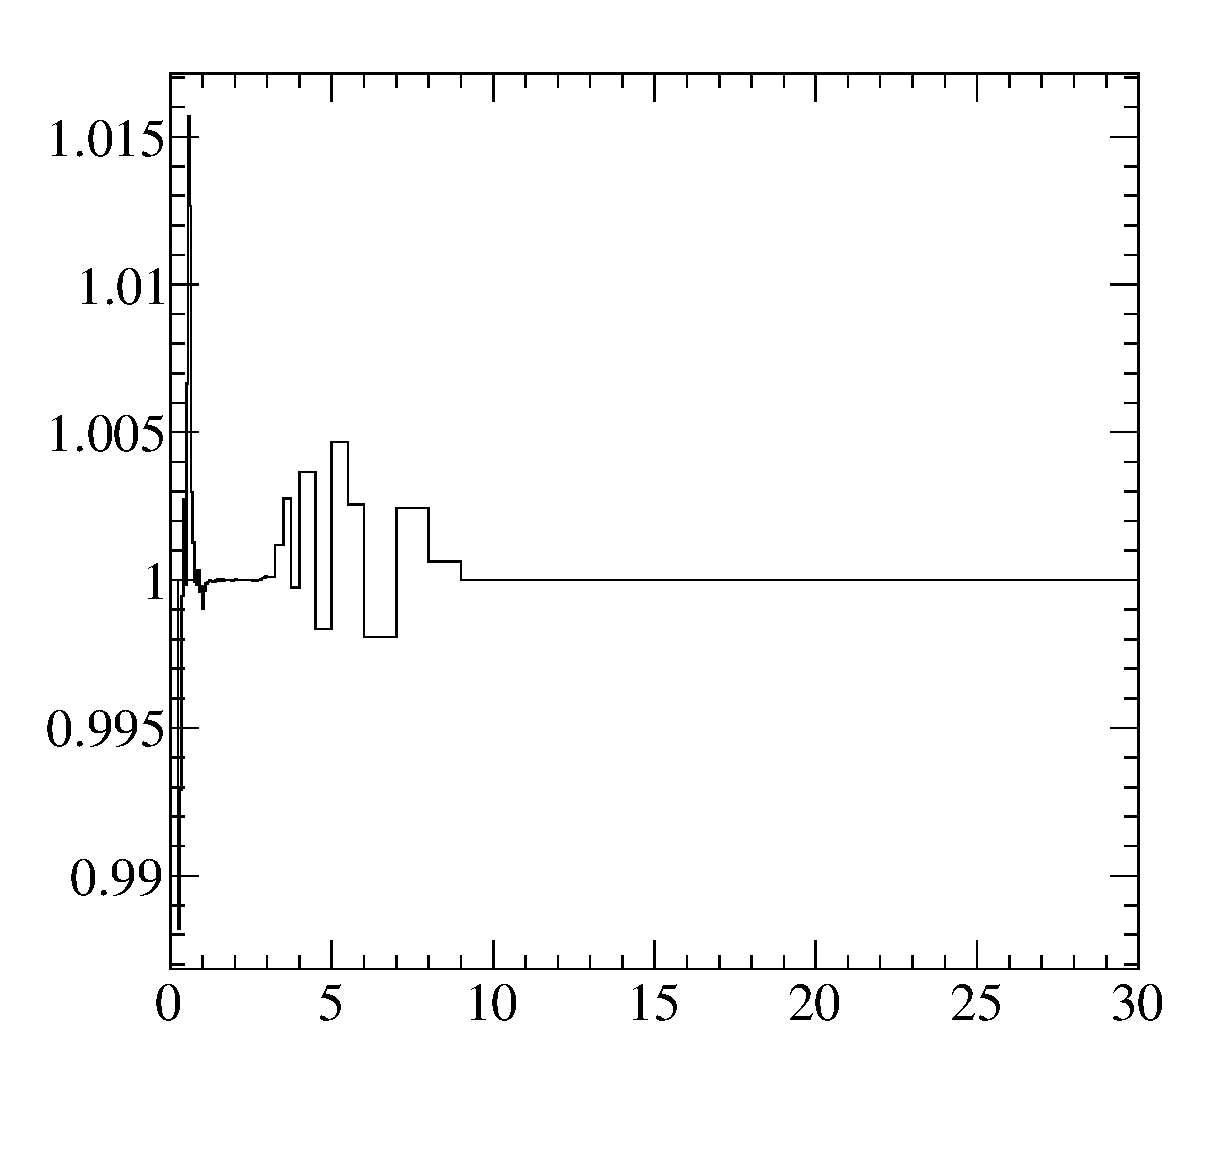
\includegraphics[width=18pc]{./images/binning/oscillation/plot_erec_int_numb_ccqe_fine}
\caption
 {Ratio of SuperK MC $E_{reco}$ spectra, for mode $\bar{\nu_\mu}$ CCQE made with 84 bin $E_{true}$ and 780 bin $E_{true}$, for an exposure of 3.010$	imes$10$^{20}$ POT. The number of events was calculated using the BANFF-tuned MC templates.Using oscillation parameters:  $\sin^22\theta_{12} = $0.857; $\sin^22\theta_{13} = $0.098; $\sin^22\theta_{23} = $1; $\delta_{CP} = $        0; $\Delta m^2_{21} = $    7.5e-05 $eV^2/c^4$; $|\Delta m^2_{32}| = $    0.0024 $eV^2/c^4$. }
\label{fig:etruebin:numubarccqe}
\end{minipage}
\hspace{0.06\linewidth}
\begin{minipage}[t]{0.48\linewidth}
\center
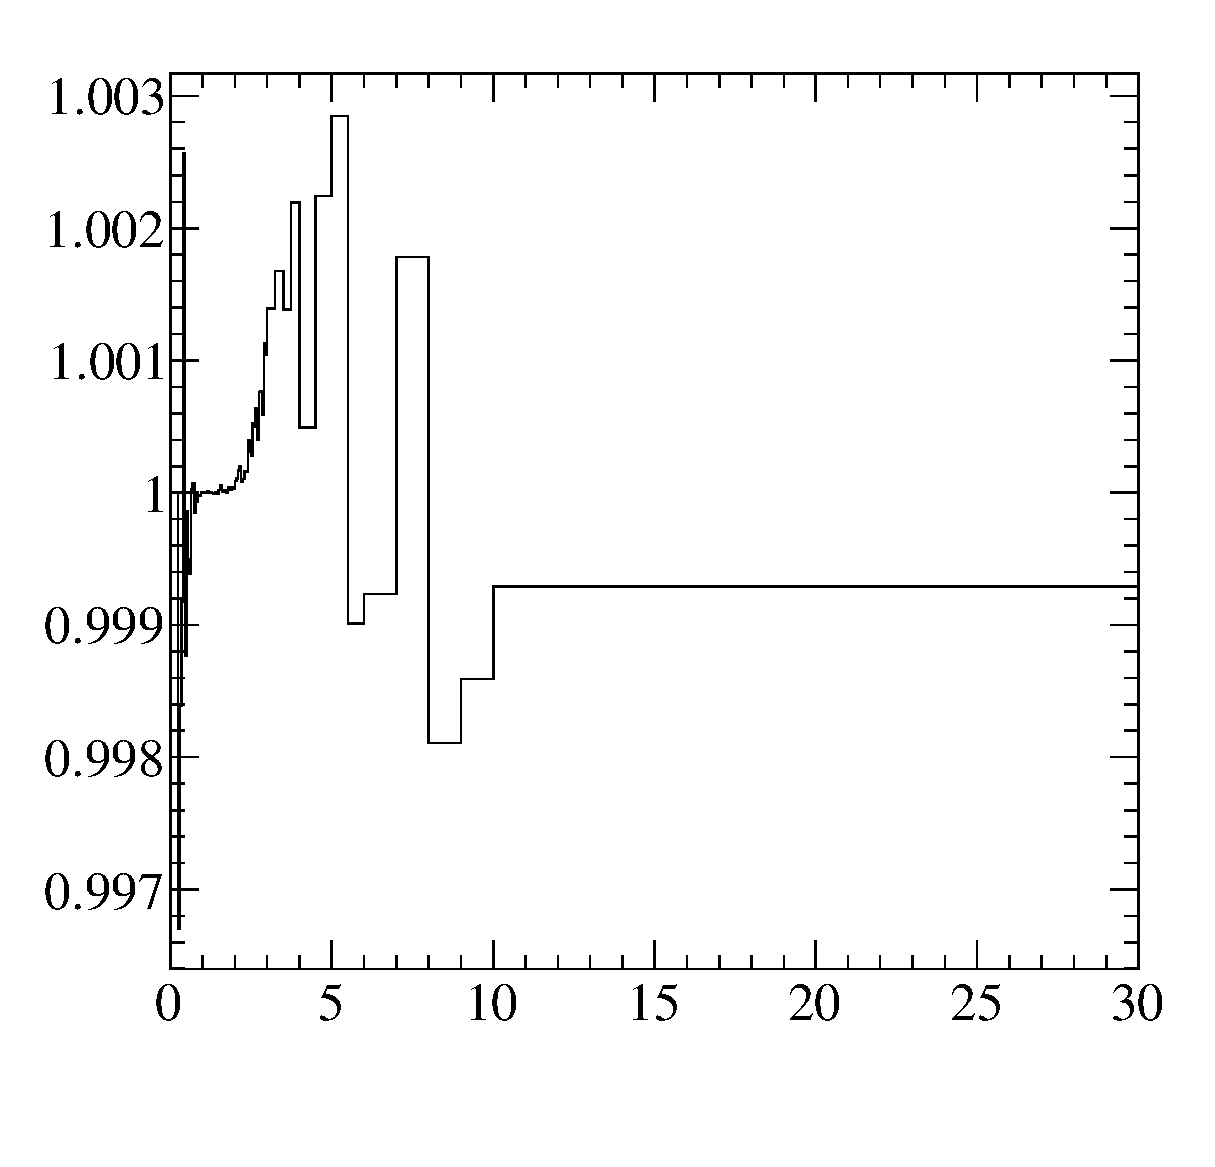
\includegraphics[width=18pc]{./images/binning/oscillation/plot_erec_int_numb_ccpi_fine}
\caption
 {Ratio of SuperK MC $E_{reco}$ spectra, for mode $\bar{\nu_\mu}$ CC 1$\pi$ made with 84 bin $E_{true}$ and 780 bin $E_{true}$, for an exposure of 3.010$	imes$10$^{20}$ POT. The number of events was calculated using the BANFF-tuned MC templates.Using oscillation parameters:  $\sin^22\theta_{12} = $0.857; $\sin^22\theta_{13} = $0.098; $\sin^22\theta_{23} = $1; $\delta_{CP} = $        0; $\Delta m^2_{21} = $    7.5e-05 $eV^2/c^4$; $|\Delta m^2_{32}| = $    0.0024 $eV^2/c^4$. }
\label{fig:etruebin:numubarcc1pi}
\end{minipage}
\vfill
\begin{minipage}[t]{0.48\linewidth}
\center
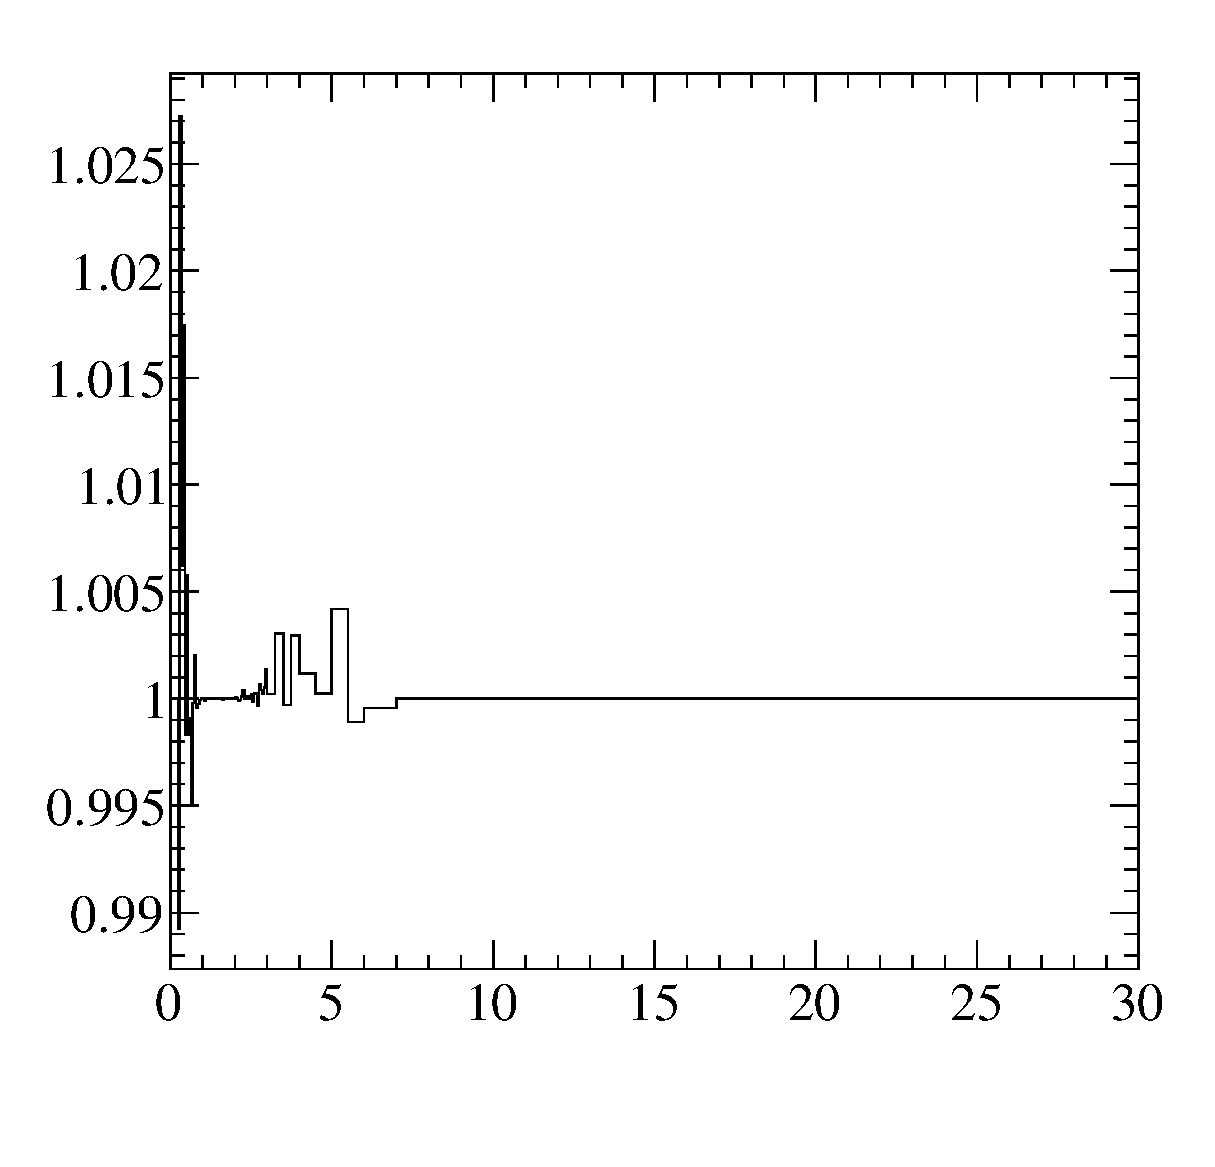
\includegraphics[width=18pc]{./images/binning/oscillation/plot_erec_int_numb_cccoh_fine}
\caption
 {Ratio of SuperK MC $E_{reco}$ spectra, for mode $\bar{\nu_\mu}$ CC coherent made with 84 bin $E_{true}$ and 780 bin $E_{true}$, for an exposure of 3.010$	imes$10$^{20}$ POT. The number of events was calculated using the BANFF-tuned MC templates.Using oscillation parameters:  $\sin^22\theta_{12} = $0.857; $\sin^22\theta_{13} = $0.098; $\sin^22\theta_{23} = $1; $\delta_{CP} = $        0; $\Delta m^2_{21} = $    7.5e-05 $eV^2/c^4$; $|\Delta m^2_{32}| = $    0.0024 $eV^2/c^4$. }
\label{fig:etruebin:numubarcccoh}
\end{minipage}
\hspace{0.06\linewidth}
\begin{minipage}[t]{0.48\linewidth}
\center
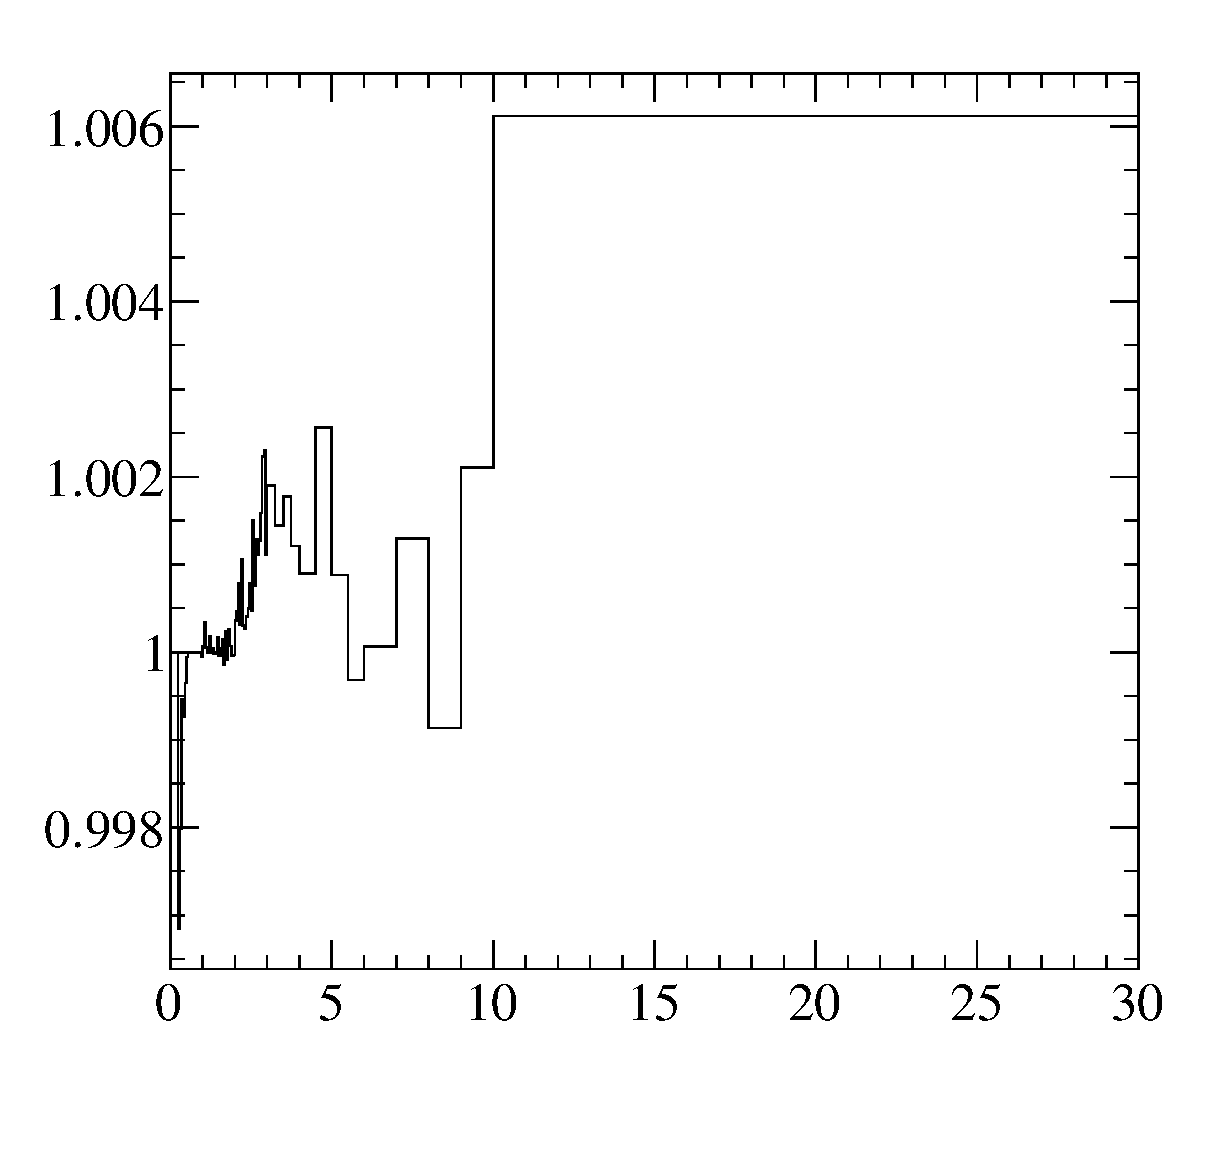
\includegraphics[width=18pc]{./images/binning/oscillation/plot_erec_int_numb_ccoth_fine}
\caption
 {Ratio of SuperK MC $E_{reco}$ spectra, for mode $\bar{\nu_\mu}$ CC other ($\nu_\mu$ disap) made with 84 bin $E_{true}$ and 780 bin $E_{true}$, for an exposure of 3.010$	imes$10$^{20}$ POT. The number of events was calculated using the BANFF-tuned MC templates.Using oscillation parameters:  $\sin^22\theta_{12} = $0.857; $\sin^22\theta_{13} = $0.098; $\sin^22\theta_{23} = $1; $\delta_{CP} = $        0; $\Delta m^2_{21} = $    7.5e-05 $eV^2/c^4$; $|\Delta m^2_{32}| = $    0.0024 $eV^2/c^4$. }
\label{fig:etruebin:numubarccoth}
\end{minipage}
\end{figure*}

%\clearpage
\begin{figure*}[htb]
\begin{minipage}[t]{0.48\linewidth}
\center
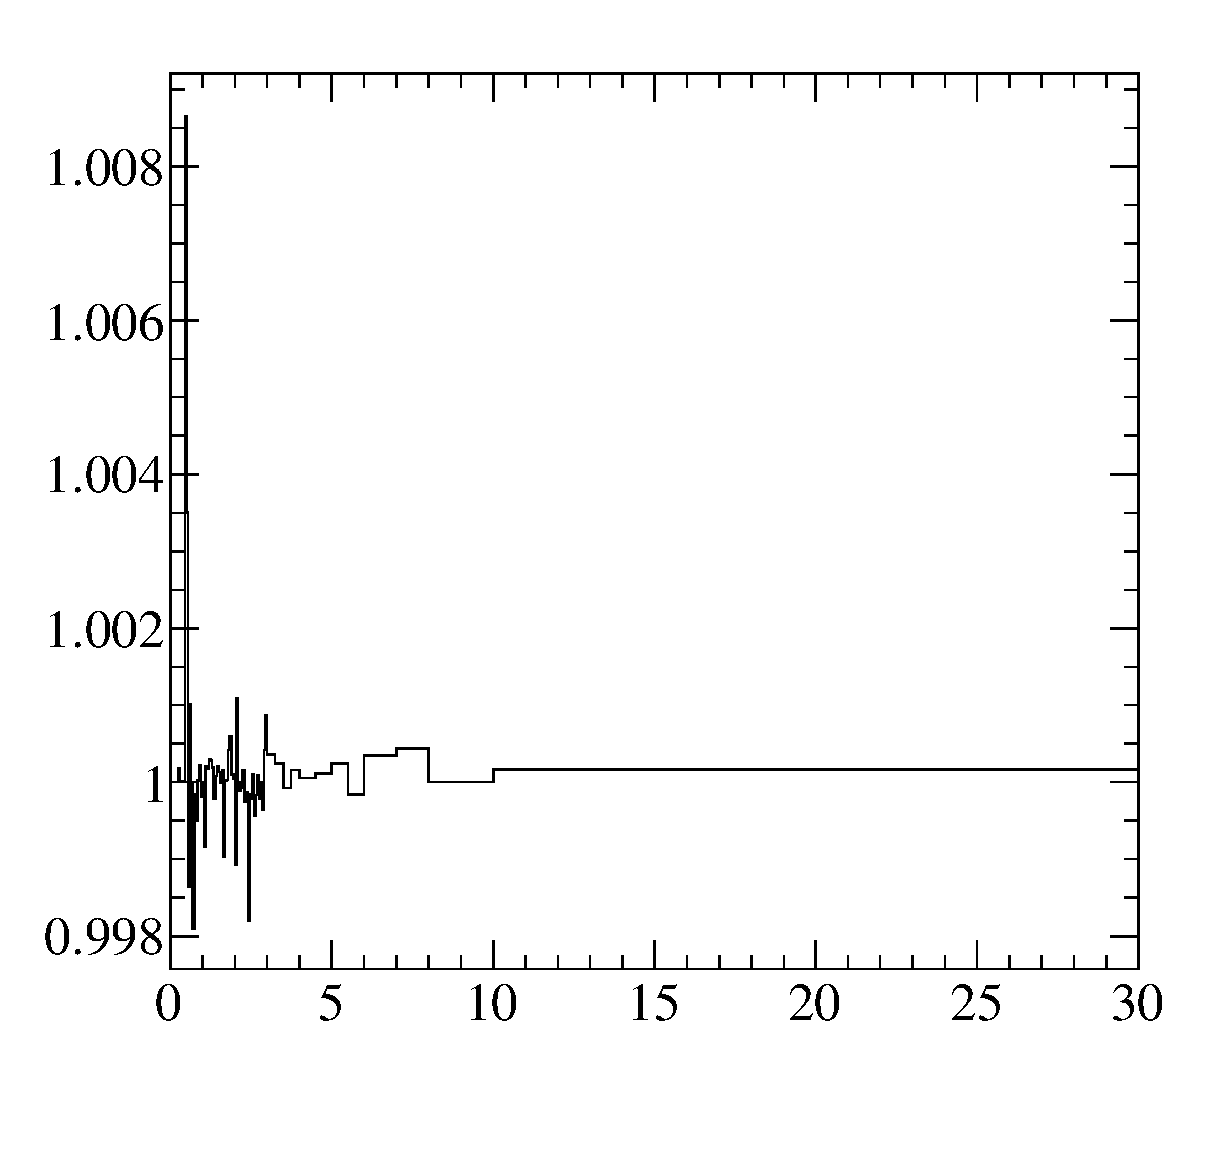
\includegraphics[width=18pc]{./images/binning/oscillation/plot_erec_int_nue_ccqe_fine}
\caption
 {Ratio of SuperK MC $E_{reco}$ spectra, for mode $\nu_e$ CCQE made with 84 bin $E_{true}$ and 780 bin $E_{true}$, for an exposure of 3.010$	imes$10$^{20}$ POT. The number of events was calculated using the BANFF-tuned MC templates.Using oscillation parameters:  $\sin^22\theta_{12} = $0.857; $\sin^22\theta_{13} = $0.098; $\sin^22\theta_{23} = $1; $\delta_{CP} = $        0; $\Delta m^2_{21} = $    7.5e-05 $eV^2/c^4$; $|\Delta m^2_{32}| = $    0.0024 $eV^2/c^4$. }
\label{fig:etruebin:nueccqe}
\end{minipage}
\hspace{0.06\linewidth}
\begin{minipage}[t]{0.48\linewidth}
\center
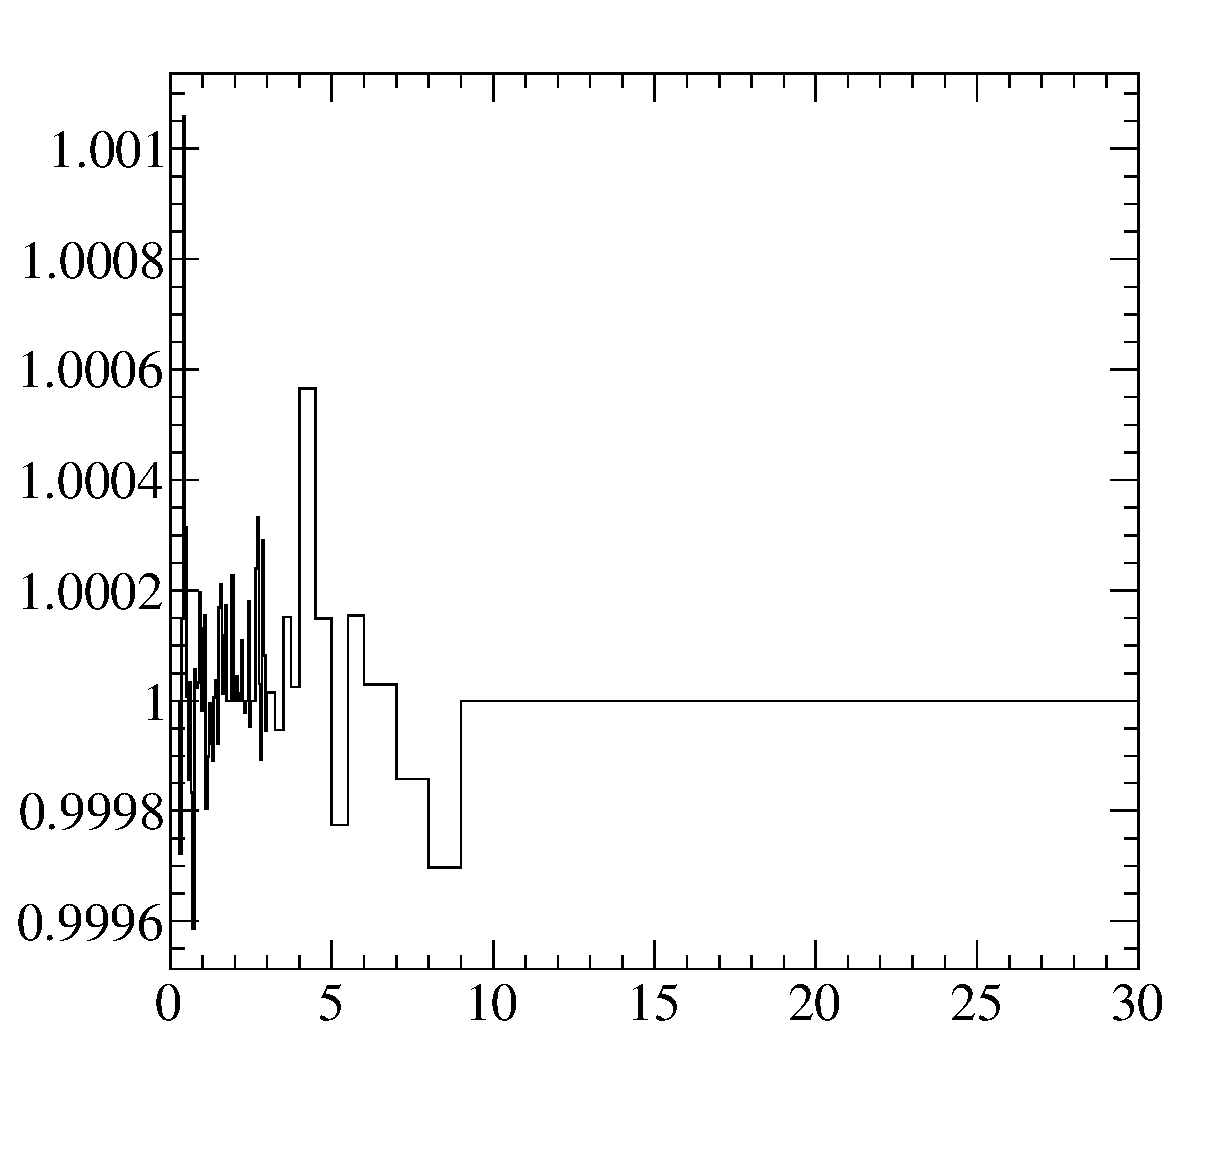
\includegraphics[width=18pc]{./images/binning/oscillation/plot_erec_int_nue_ccpi_fine}
\caption
 {Ratio of SuperK MC $E_{reco}$ spectra, for mode $\nu_e$ CC 1$\pi$ made with 84 bin $E_{true}$ and 780 bin $E_{true}$, for an exposure of 3.010$	imes$10$^{20}$ POT. The number of events was calculated using the BANFF-tuned MC templates.Using oscillation parameters:  $\sin^22\theta_{12} = $0.857; $\sin^22\theta_{13} = $0.098; $\sin^22\theta_{23} = $1; $\delta_{CP} = $        0; $\Delta m^2_{21} = $    7.5e-05 $eV^2/c^4$; $|\Delta m^2_{32}| = $    0.0024 $eV^2/c^4$. }
\label{fig:etruebin:nuecc1pi}
\end{minipage}
\vfill
\begin{minipage}[t]{0.48\linewidth}
\center
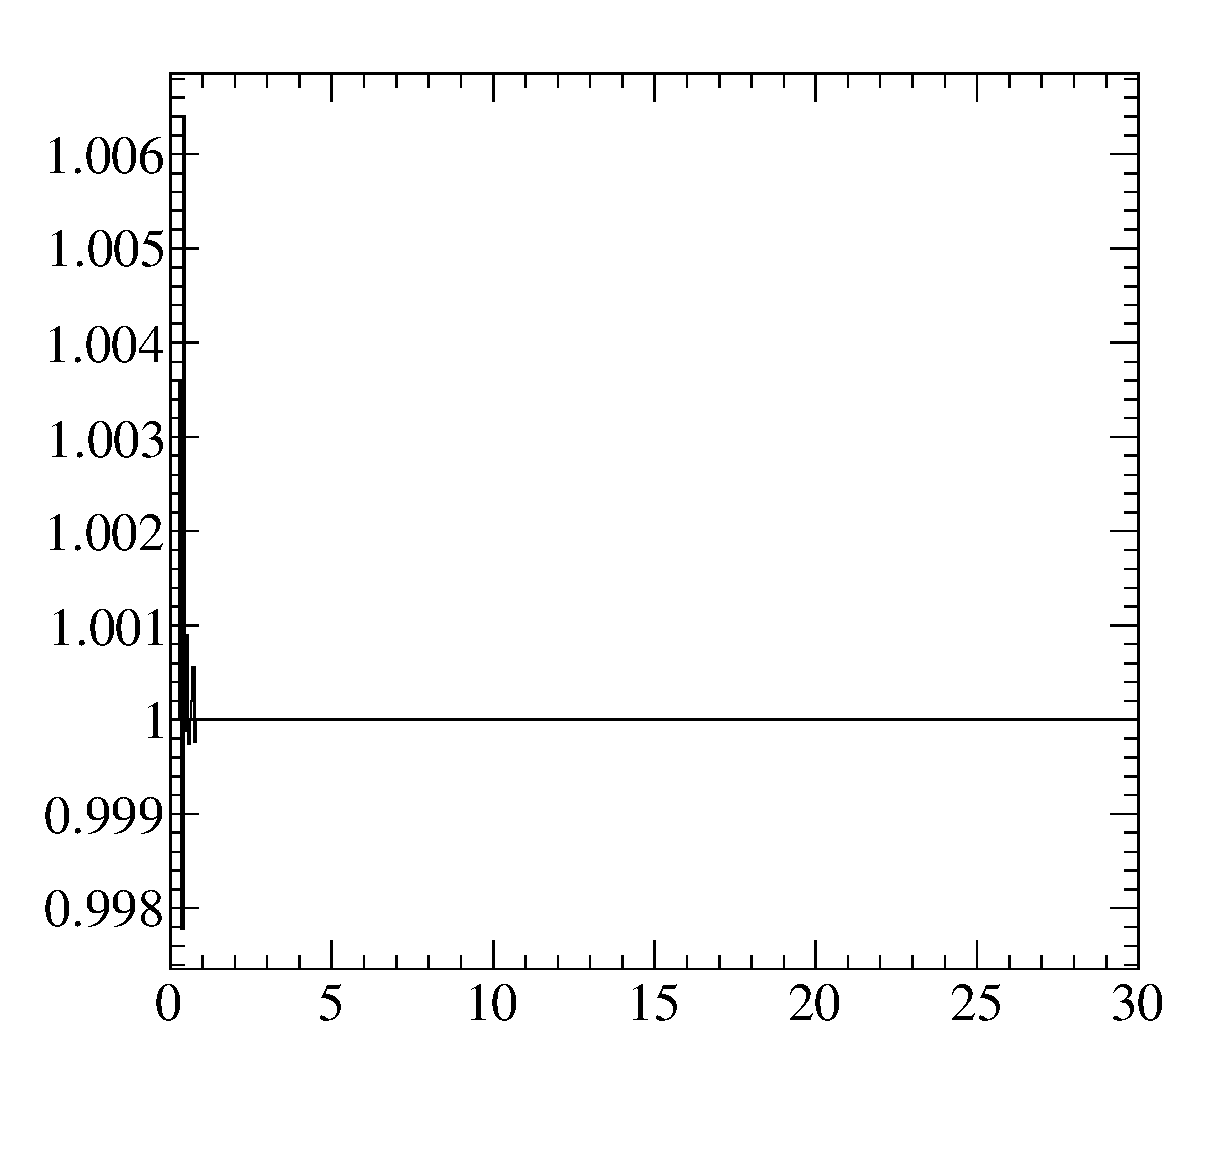
\includegraphics[width=18pc]{./images/binning/oscillation/plot_erec_int_nue_cccoh_fine}
\caption
 {Ratio of SuperK MC $E_{reco}$ spectra, for mode $\nu_e$ CC coherent made with 84 bin $E_{true}$ and 780 bin $E_{true}$, for an exposure of 3.010$	imes$10$^{20}$ POT. The number of events was calculated using the BANFF-tuned MC templates.Using oscillation parameters:  $\sin^22\theta_{12} = $0.857; $\sin^22\theta_{13} = $0.098; $\sin^22\theta_{23} = $1; $\delta_{CP} = $        0; $\Delta m^2_{21} = $    7.5e-05 $eV^2/c^4$; $|\Delta m^2_{32}| = $    0.0024 $eV^2/c^4$. }
\label{fig:etruebin:nuecccoh}
\end{minipage}
\hspace{0.06\linewidth}
\begin{minipage}[t]{0.48\linewidth}
\center
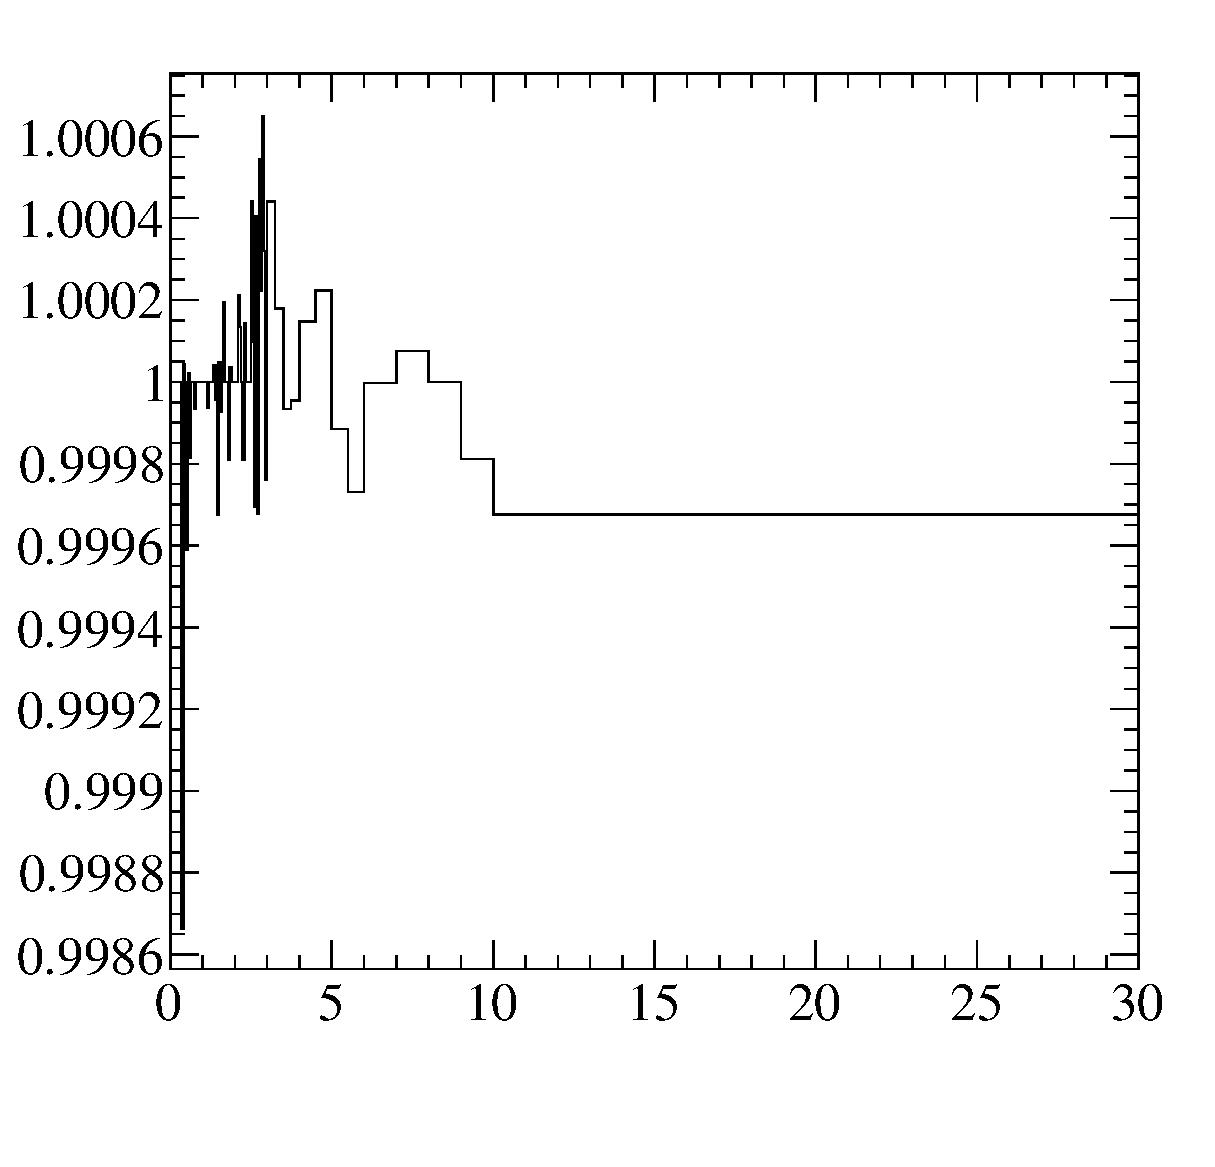
\includegraphics[width=18pc]{./images/binning/oscillation/plot_erec_int_nue_ccoth_fine}
\caption
 {Ratio of SuperK MC $E_{reco}$ spectra, for mode $\nu_e$ CC other ($\nu_\mu$ disap) made with 84 bin $E_{true}$ and 780 bin $E_{true}$, for an exposure of 3.010$	imes$10$^{20}$ POT. The number of events was calculated using the BANFF-tuned MC templates.Using oscillation parameters:  $\sin^22\theta_{12} = $0.857; $\sin^22\theta_{13} = $0.098; $\sin^22\theta_{23} = $1; $\delta_{CP} = $        0; $\Delta m^2_{21} = $    7.5e-05 $eV^2/c^4$; $|\Delta m^2_{32}| = $    0.0024 $eV^2/c^4$. }
\label{fig:etruebin:nueccoth}
\end{minipage}
\end{figure*}

%\clearpage
\begin{figure*}[htb]
\begin{minipage}[t]{0.48\linewidth}
\center
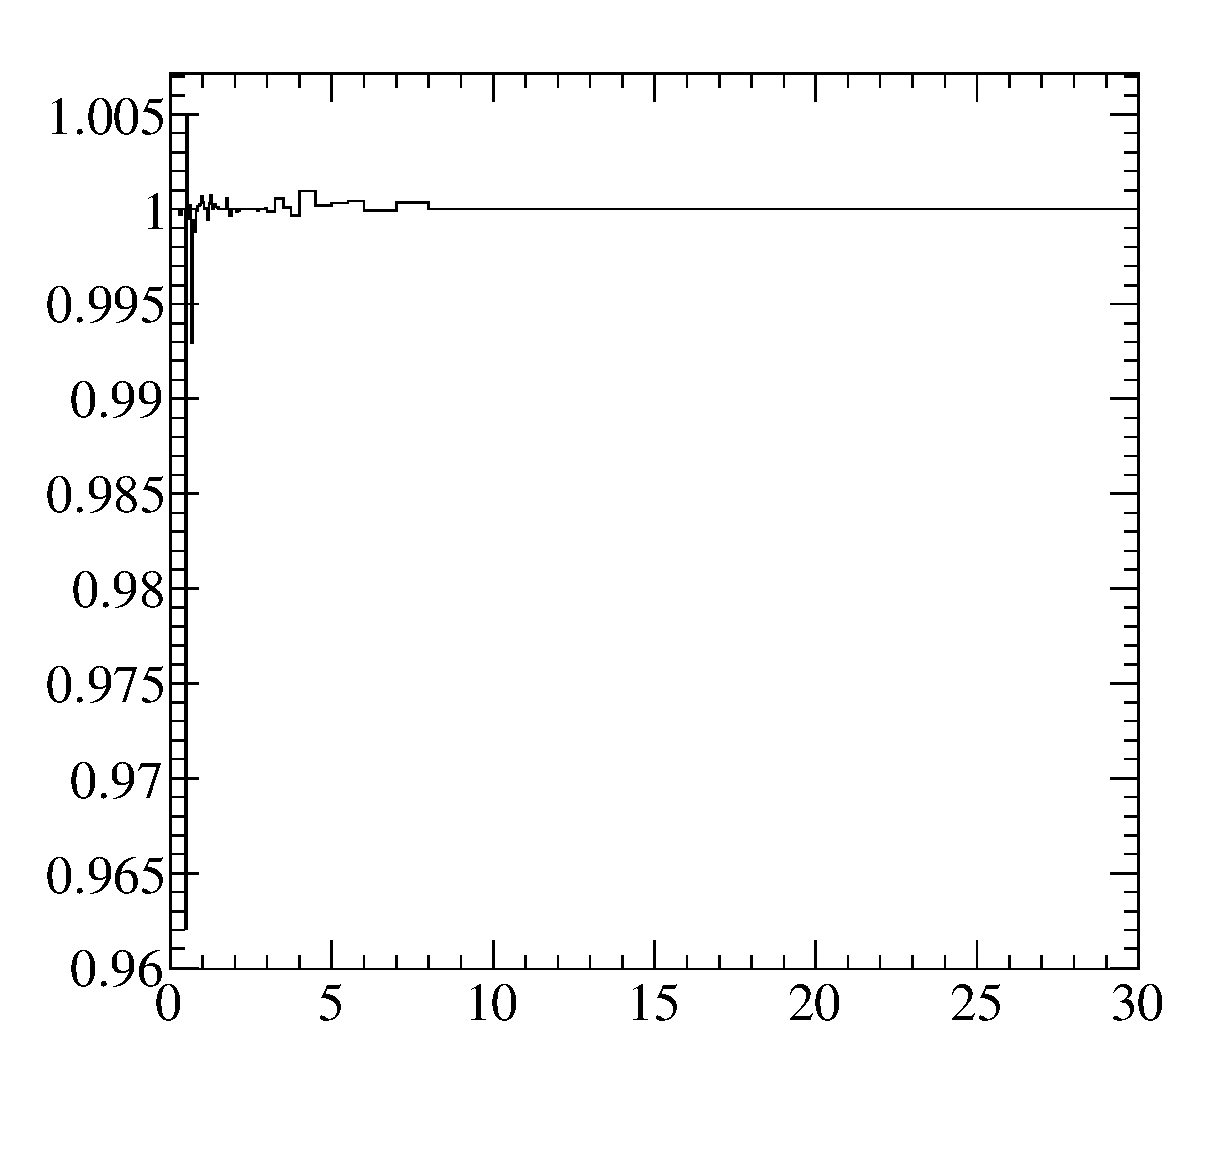
\includegraphics[width=18pc]{./images/binning/oscillation/plot_erec_int_nueb_ccqe_fine}
\caption
 {Ratio of SuperK MC $E_{reco}$ spectra, for mode $\bar{\nu_e}$ CCQE made with 84 bin $E_{true}$ and 780 bin $E_{true}$, for an exposure of 3.010$	imes$10$^{20}$ POT. The number of events was calculated using the BANFF-tuned MC templates.Using oscillation parameters:  $\sin^22\theta_{12} = $0.857; $\sin^22\theta_{13} = $0.098; $\sin^22\theta_{23} = $1; $\delta_{CP} = $        0; $\Delta m^2_{21} = $    7.5e-05 $eV^2/c^4$; $|\Delta m^2_{32}| = $    0.0024 $eV^2/c^4$. }
\label{fig:etruebin:nuebarccqe}
\end{minipage}
\hspace{0.06\linewidth}
\begin{minipage}[t]{0.48\linewidth}
\center
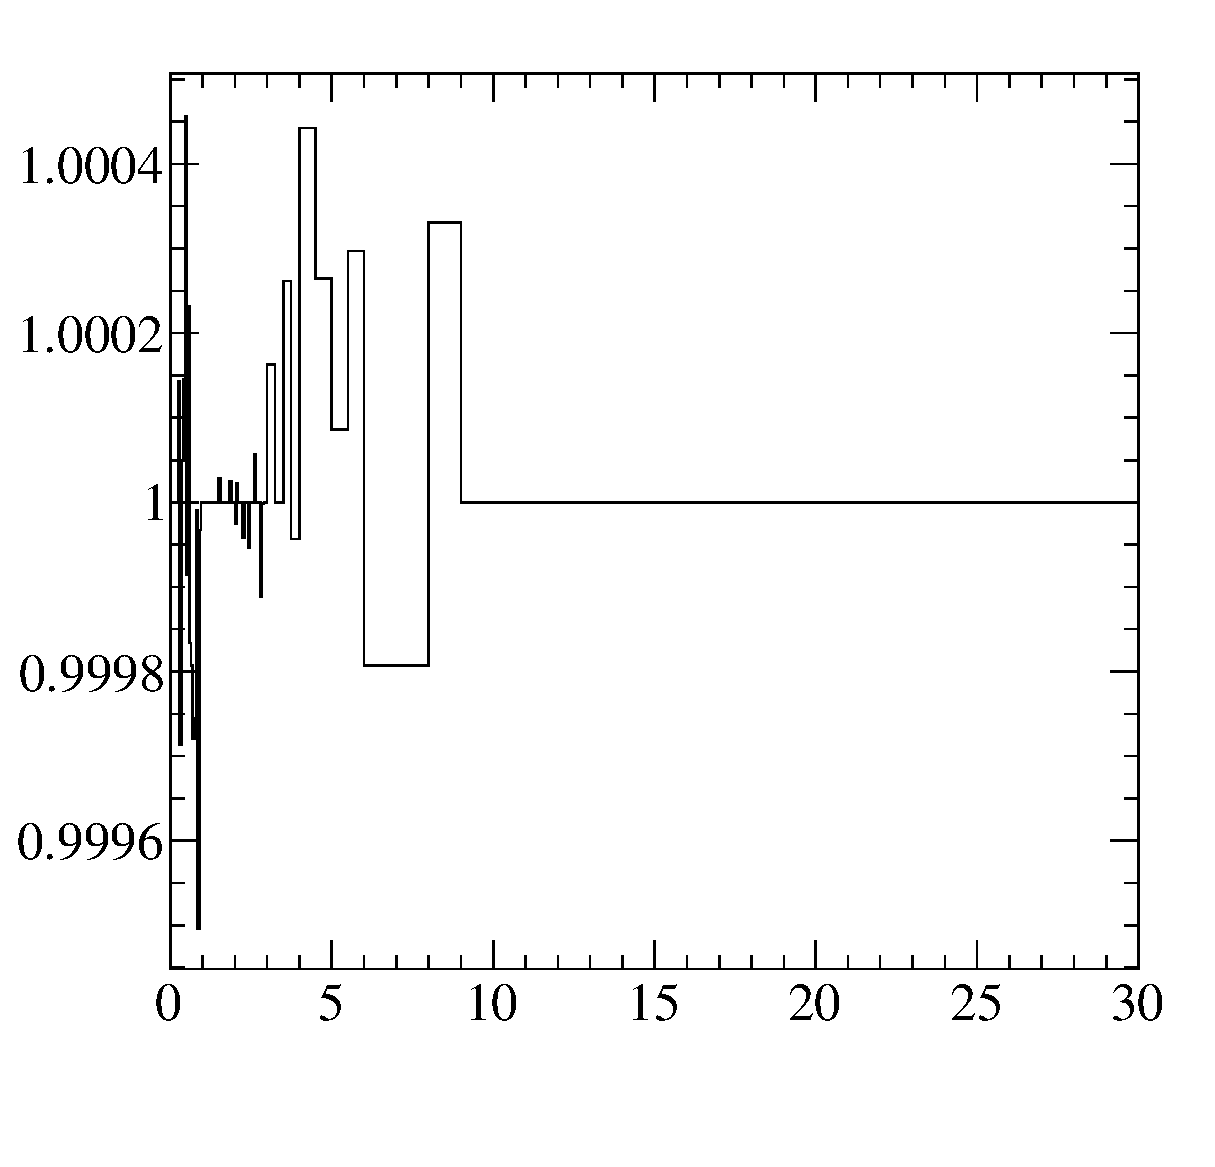
\includegraphics[width=18pc]{./images/binning/oscillation/plot_erec_int_nueb_ccpi_fine}
\caption
 {Ratio of SuperK MC $E_{reco}$ spectra, for mode $\bar{\nu_e}$ CC 1$\pi$ made with 84 bin $E_{true}$ and 780 bin $E_{true}$, for an exposure of 3.010$	imes$10$^{20}$ POT. The number of events was calculated using the BANFF-tuned MC templates.Using oscillation parameters:  $\sin^22\theta_{12} = $0.857; $\sin^22\theta_{13} = $0.098; $\sin^22\theta_{23} = $1; $\delta_{CP} = $        0; $\Delta m^2_{21} = $    7.5e-05 $eV^2/c^4$; $|\Delta m^2_{32}| = $    0.0024 $eV^2/c^4$. }
\label{fig:etruebin:nuebarcc1pi}
\end{minipage}
\vfill
\begin{minipage}[t]{0.48\linewidth}
\center
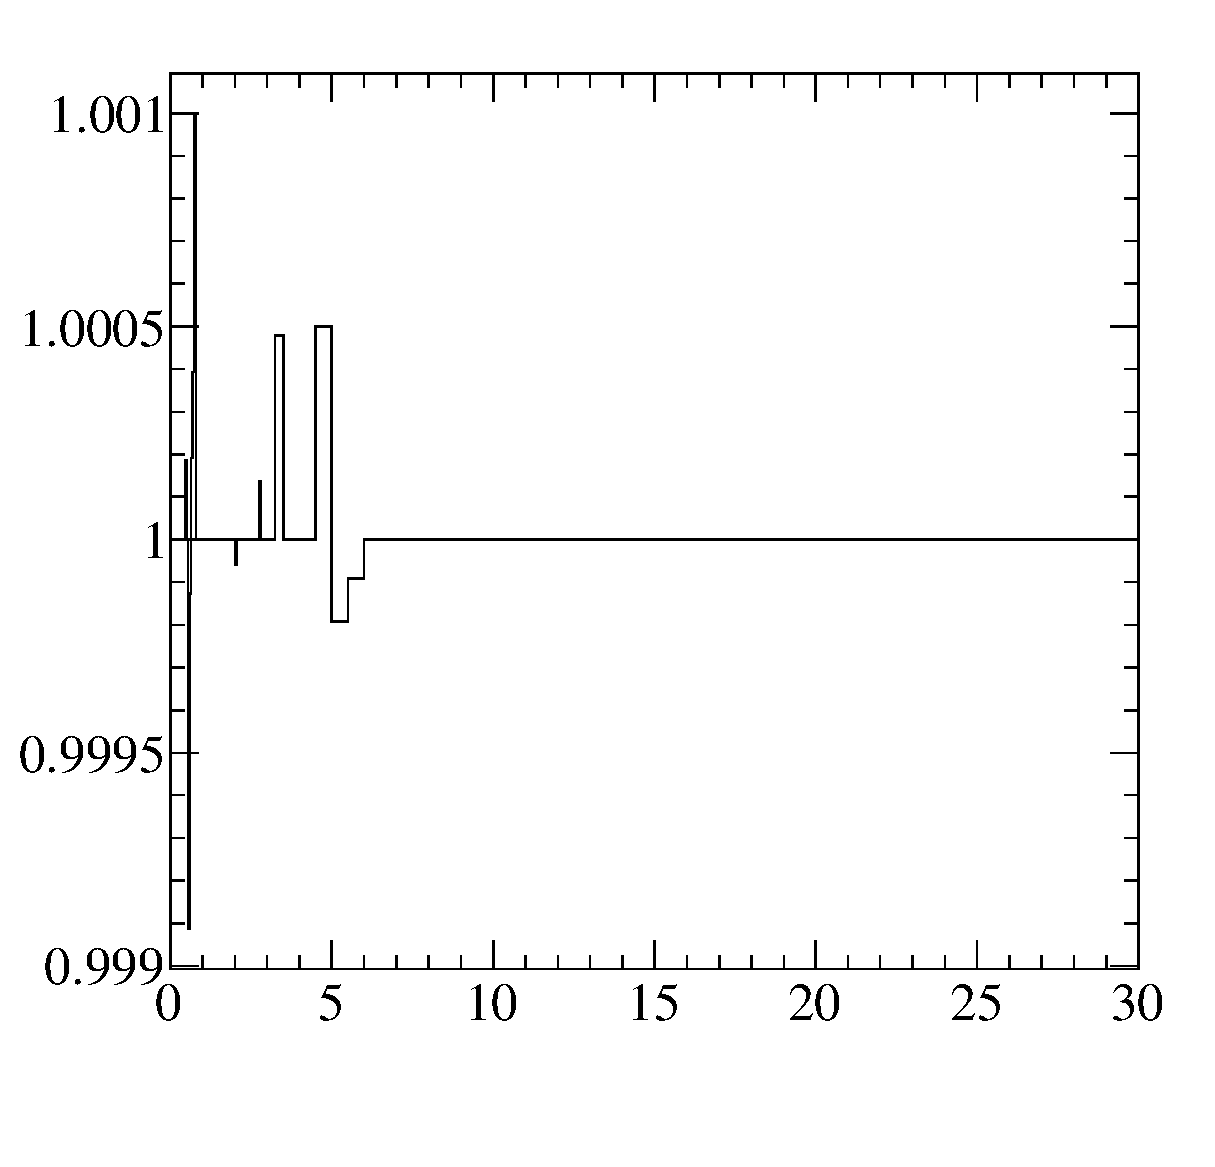
\includegraphics[width=18pc]{./images/binning/oscillation/plot_erec_int_nueb_cccoh_fine}
\caption
 {Ratio of SuperK MC $E_{reco}$ spectra, for mode $\bar{\nu_e}$ CC coherent made with 84 bin $E_{true}$ and 780 bin $E_{true}$, for an exposure of 3.010$	imes$10$^{20}$ POT. The number of events was calculated using the BANFF-tuned MC templates.Using oscillation parameters:  $\sin^22\theta_{12} = $0.857; $\sin^22\theta_{13} = $0.098; $\sin^22\theta_{23} = $1; $\delta_{CP} = $        0; $\Delta m^2_{21} = $    7.5e-05 $eV^2/c^4$; $|\Delta m^2_{32}| = $    0.0024 $eV^2/c^4$. }
\label{fig:etruebin:nuebarcccoh}
\end{minipage}
\hspace{0.06\linewidth}
\begin{minipage}[t]{0.48\linewidth}
\center
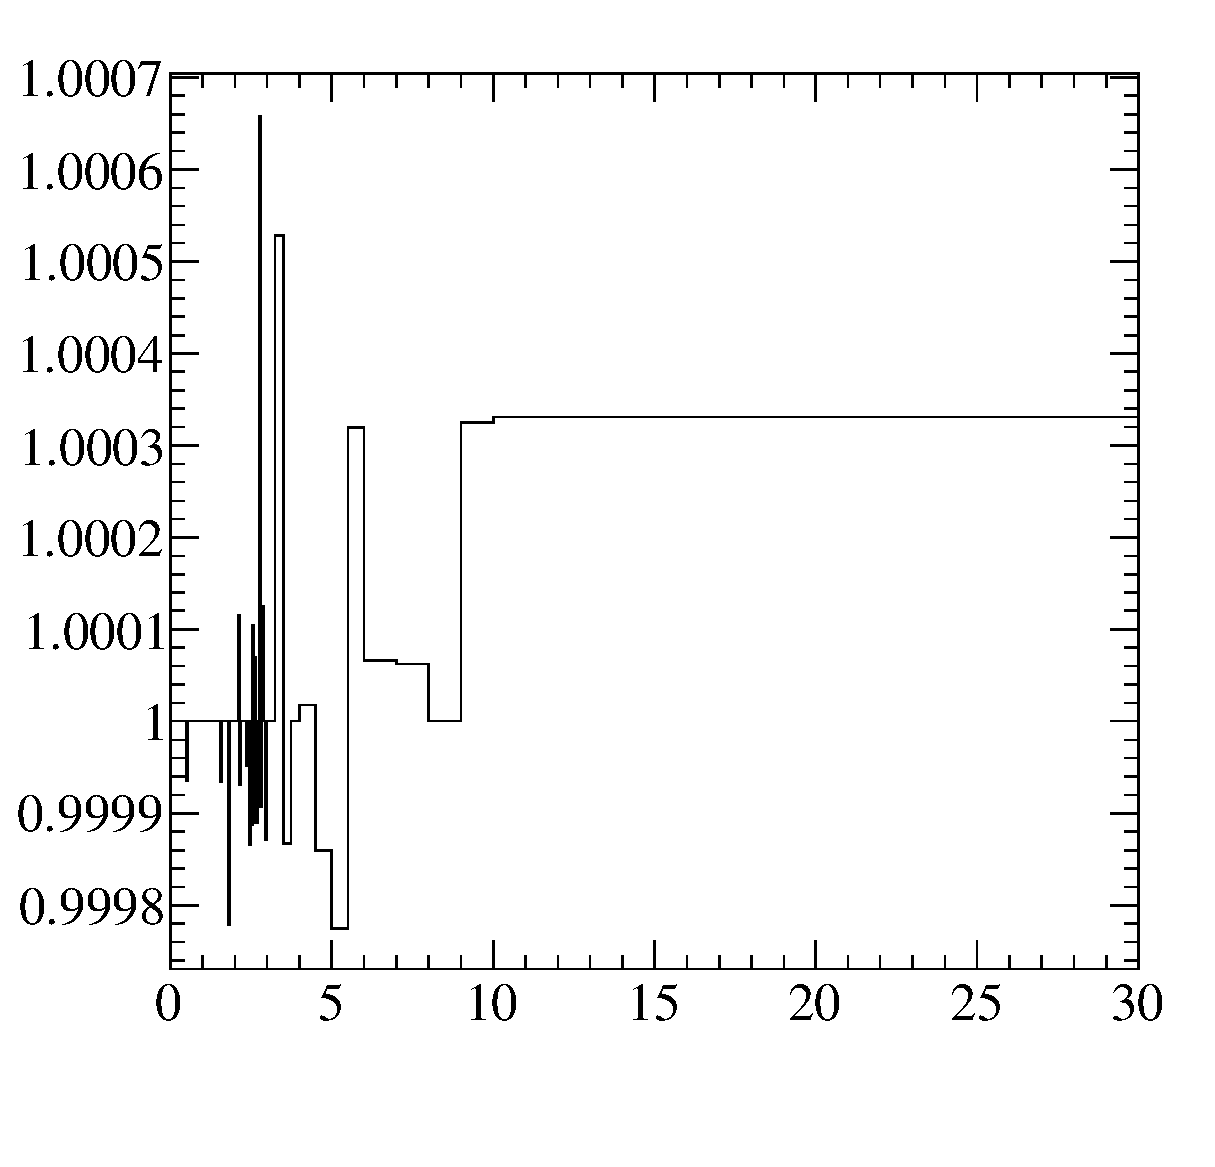
\includegraphics[width=18pc]{./images/binning/oscillation/plot_erec_int_nueb_ccoth_fine}
\caption
 {Ratio of SuperK MC $E_{reco}$ spectra, for mode $\bar{\nu_e}$ CC other ($\nu_\mu$ disap) made with 84 bin $E_{true}$ and 780 bin $E_{true}$, for an exposure of 3.010$	imes$10$^{20}$ POT. The number of events was calculated using the BANFF-tuned MC templates.Using oscillation parameters:  $\sin^22\theta_{12} = $0.857; $\sin^22\theta_{13} = $0.098; $\sin^22\theta_{23} = $1; $\delta_{CP} = $        0; $\Delta m^2_{21} = $    7.5e-05 $eV^2/c^4$; $|\Delta m^2_{32}| = $    0.0024 $eV^2/c^4$. }
\label{fig:etruebin:nuebarccoth}
\end{minipage}
\end{figure*}

%\clearpage
\begin{figure*}[htb]
\begin{minipage}[t]{0.48\linewidth}
\center
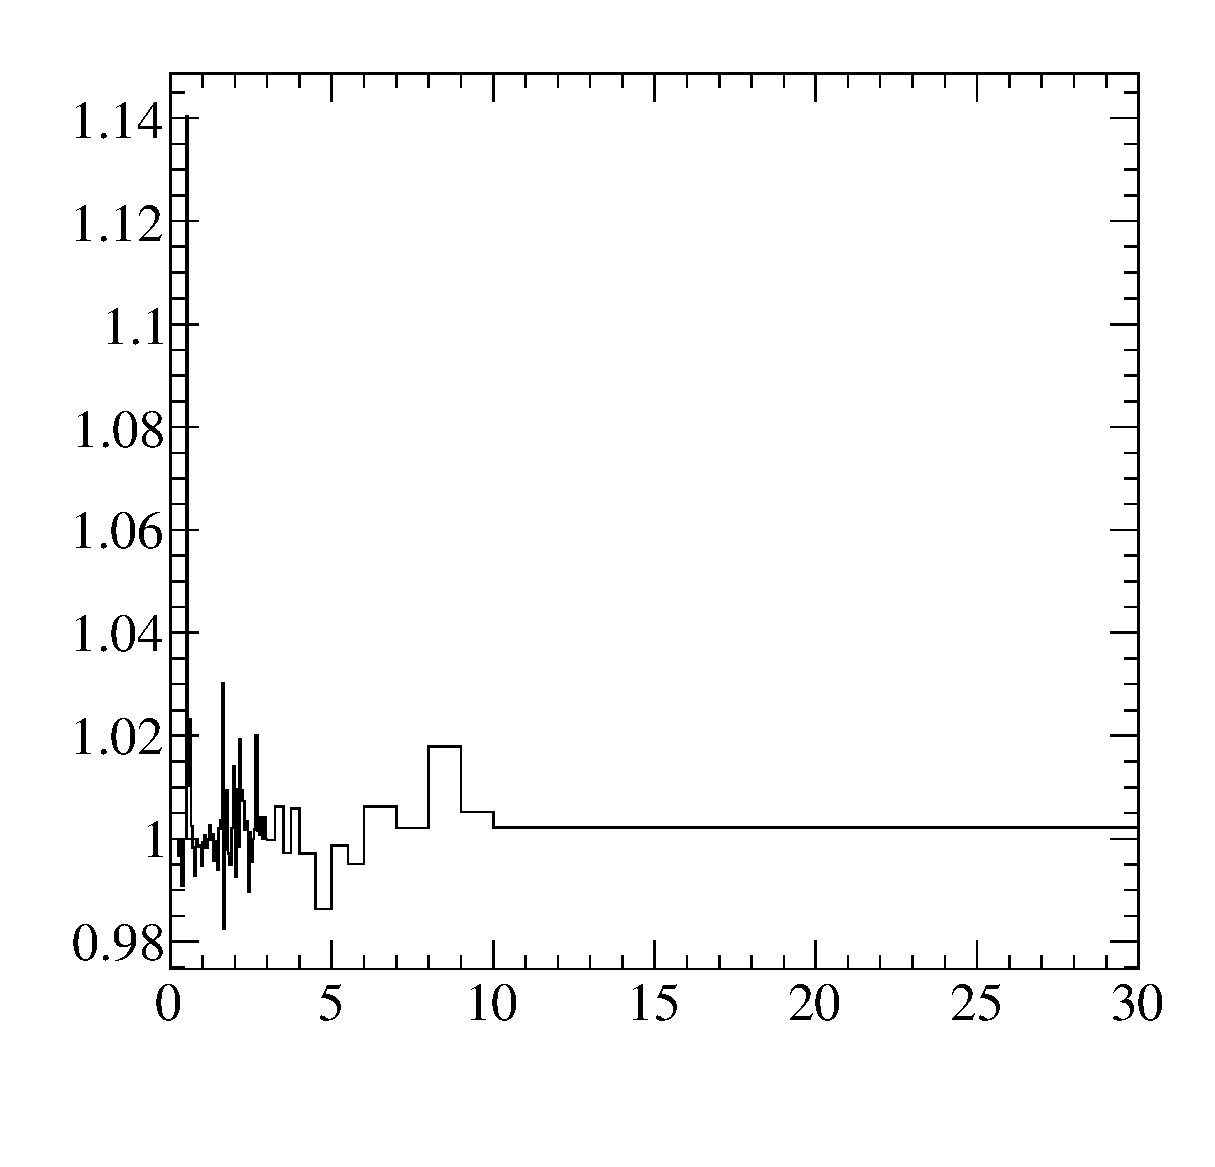
\includegraphics[width=18pc]{./images/binning/oscillation/plot_erec_int_signue_ccqe_fine}
\caption
 {Ratio of SuperK MC $E_{reco}$ spectra, for mode oscillation $\nu_e$ CCQE made with 84 bin $E_{true}$ and 780 bin $E_{true}$, for an exposure of 3.010$	imes$10$^{20}$ POT. The number of events was calculated using the BANFF-tuned MC templates.Using oscillation parameters:  $\sin^22\theta_{12} = $0.857; $\sin^22\theta_{13} = $0.098; $\sin^22\theta_{23} = $1; $\delta_{CP} = $        0; $\Delta m^2_{21} = $    7.5e-05 $eV^2/c^4$; $|\Delta m^2_{32}| = $    0.0024 $eV^2/c^4$. }
\label{fig:etruebin:signueccqe}
\end{minipage}
\hspace{0.06\linewidth}
\begin{minipage}[t]{0.48\linewidth}
\center
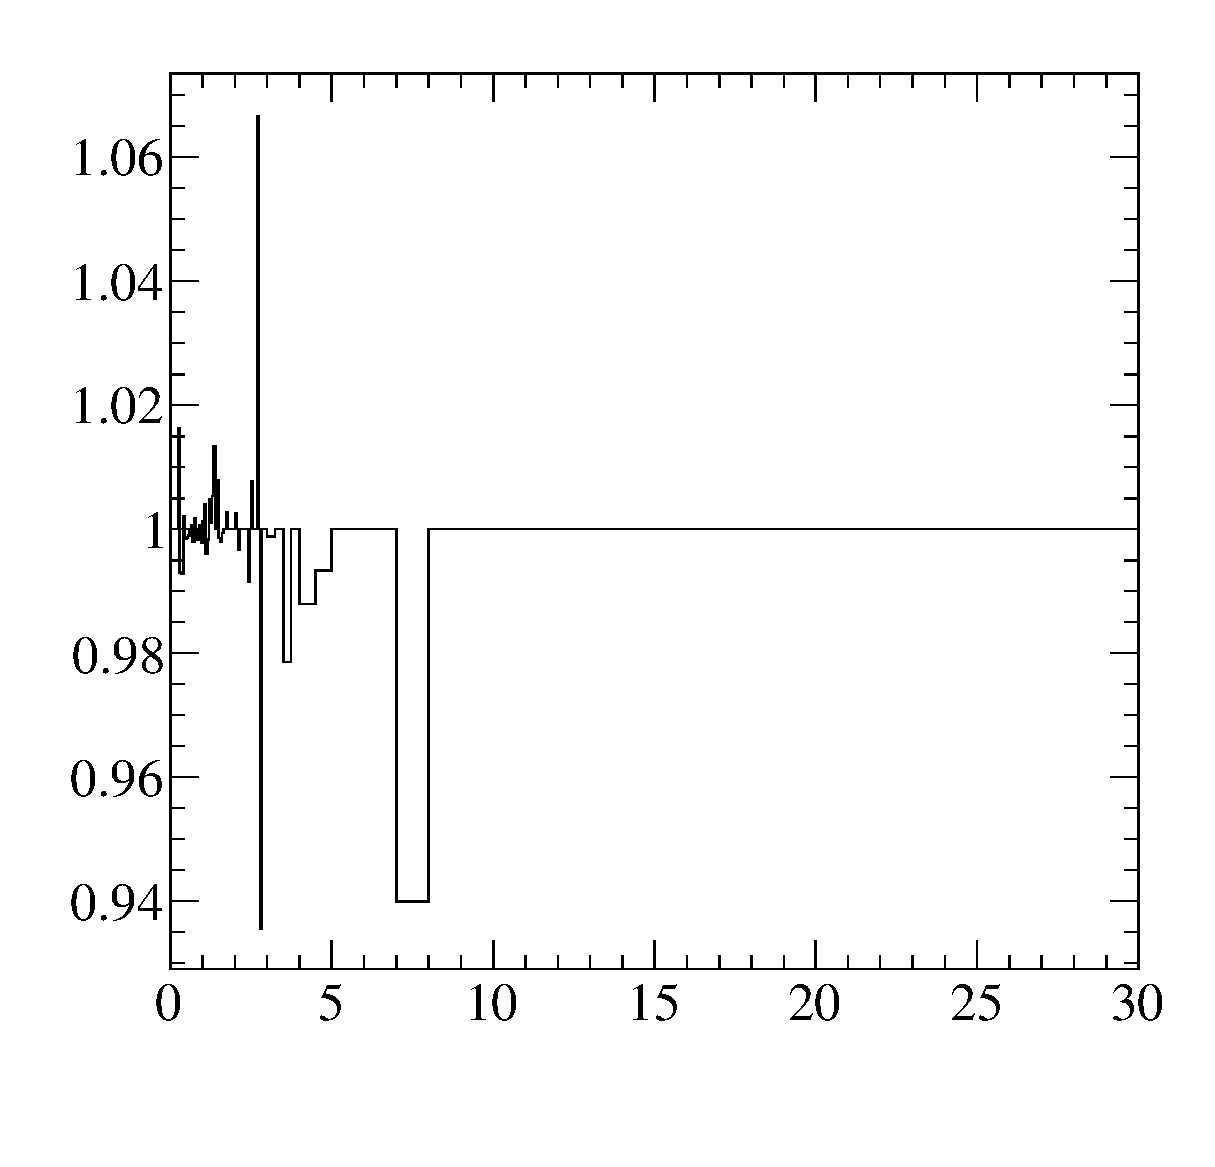
\includegraphics[width=18pc]{./images/binning/oscillation/plot_erec_int_signue_ccpi_fine}
\caption
 {Ratio of SuperK MC $E_{reco}$ spectra, for mode oscillation $\nu_e$ CC 1$\pi$ made with 84 bin $E_{true}$ and 780 bin $E_{true}$, for an exposure of 3.010$	imes$10$^{20}$ POT. The number of events was calculated using the BANFF-tuned MC templates.Using oscillation parameters:  $\sin^22\theta_{12} = $0.857; $\sin^22\theta_{13} = $0.098; $\sin^22\theta_{23} = $1; $\delta_{CP} = $        0; $\Delta m^2_{21} = $    7.5e-05 $eV^2/c^4$; $|\Delta m^2_{32}| = $    0.0024 $eV^2/c^4$. }
\label{fig:etruebin:signuecc1pi}
\end{minipage}
\vfill
\begin{minipage}[t]{0.48\linewidth}
\center
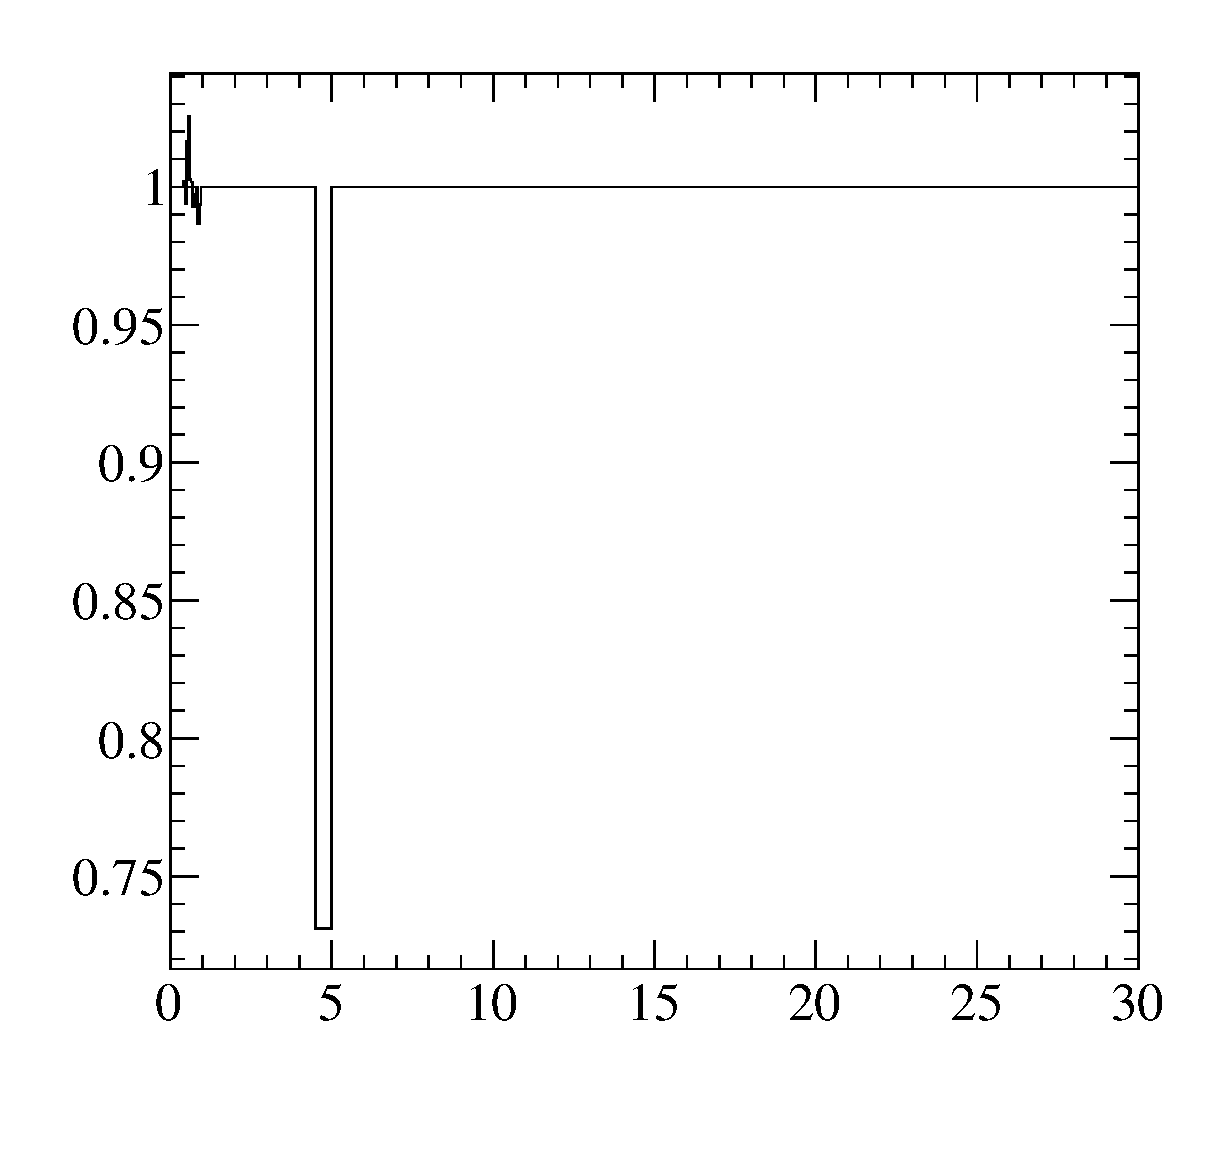
\includegraphics[width=18pc]{./images/binning/oscillation/plot_erec_int_signue_cccoh_fine}
\caption
 {Ratio of SuperK MC $E_{reco}$ spectra, for mode oscillation $\nu_e$ CC coherent made with 84 bin $E_{true}$ and 780 bin $E_{true}$, for an exposure of 3.010$	imes$10$^{20}$ POT. The number of events was calculated using the BANFF-tuned MC templates.Using oscillation parameters:  $\sin^22\theta_{12} = $0.857; $\sin^22\theta_{13} = $0.098; $\sin^22\theta_{23} = $1; $\delta_{CP} = $        0; $\Delta m^2_{21} = $    7.5e-05 $eV^2/c^4$; $|\Delta m^2_{32}| = $    0.0024 $eV^2/c^4$. }
\label{fig:etruebin:signuecccoh}
\end{minipage}
\hspace{0.06\linewidth}
\begin{minipage}[t]{0.48\linewidth}
\center
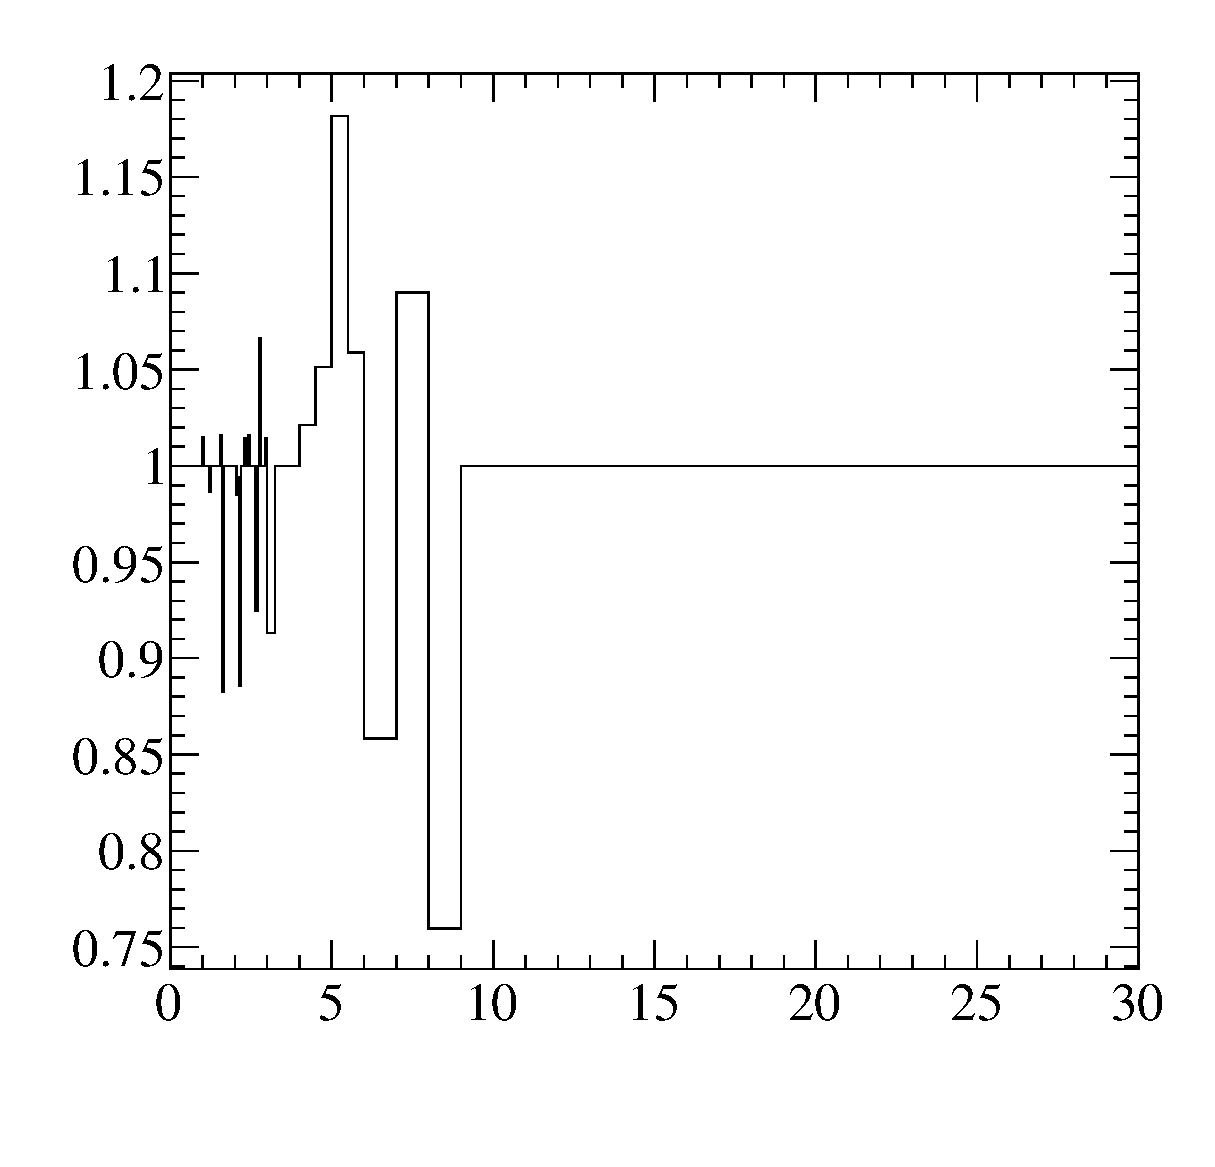
\includegraphics[width=18pc]{./images/binning/oscillation/plot_erec_int_signue_ccoth_fine}
\caption
 {Ratio of SuperK MC $E_{reco}$ spectra, for mode oscillation $\nu_e$ CC other ($\nu_\mu$ app) made with 84 bin $E_{true}$ and 780 bin $E_{true}$, for an exposure of 3.010$	imes$10$^{20}$ POT. The number of events was calculated using the BANFF-tuned MC templates.Using oscillation parameters:  $\sin^22\theta_{12} = $0.857; $\sin^22\theta_{13} = $0.098; $\sin^22\theta_{23} = $1; $\delta_{CP} = $        0; $\Delta m^2_{21} = $    7.5e-05 $eV^2/c^4$; $\Delta m^2_{32} = $    0.0024 $eV^2/c^4$. }
\label{fig:etruebin:signueccoth}
\end{minipage}
\end{figure*}

\clearpage
